\documentclass[11pt,a4paper]{article}
\usepackage[utf8]{inputenc}
\usepackage[T1]{fontenc}
\usepackage[spanish,es-noquoting,es-nodecimaldot]{babel}
\usepackage{amsmath,amssymb,bm,slashed}
\usepackage{booktabs,longtable}
\usepackage{graphicx}
\usepackage[margin=2.3cm]{geometry}
\usepackage[colorlinks=true,linkcolor=blue!60!black,citecolor=blue!60!black,urlcolor=blue!60!black]{hyperref}
\usepackage{xcolor}
\newcommand{\Ap}{A'}
\newcommand{\eps}{\epsilon}
\newcommand{\KN}{\mathrm{KN}}
\newcommand{\dd}{\mathrm{d}}
\newcommand{\wpr}{\omega'}

\title{Correcciones a la sección eficaz de producción de fotones oscuros\\[4pt]
\large Explicaciones paso a paso, una sección por pregunta}
\author{E.~L.~De Paoli\\[2pt]\small escrito con asistencia de agentes (Claude Opus 5)}
\date{Documento vivo. Última actualización: 23 de septiembre de 2026 (sección 3)}

\begin{document}
\maketitle

\noindent\sloppy
Este documento acompaña a \texttt{mycodes/DP3\_Danilov\_new.C} y a
\texttt{reports/report\_cross\_section\_es.pdf}. Cada sección responde una pregunta concreta sobre por qué la
sección eficaz del apunte \texttt{Dark\_Photon\_cross\_section-1.pdf} necesita corrección y qué cambia al corregirla.
Se agregan secciones a medida que surgen las preguntas. Todos los números salen de
\texttt{work/check\_cross\_section.py} y de \texttt{mycodes/run\_new.log}; están registrados en
\texttt{provenance/numbers.json}.

\medskip
\noindent\textbf{Notación} (la del apunte): $\omega$ = energía del fotón incidente, $\wpr$ = energía del fotón oscuro,
$m_e$ = masa del electrón, $M \equiv m_{\Ap}$. Denominadores de propagador:
$a \equiv s-m_e^2 = 2m_e\omega$, $b \equiv u-m_e^2 = M^2-2m_e\wpr$.

\tableofcontents

%=====================================================================================================
\section{¿La discontinuidad en \texorpdfstring{$m_{\Ap}=1$}{mA'=1} MeV de la Figura 1 se debe a la aproximación \texorpdfstring{$|\vec k'|\approx\wpr$}{|k'| ~ w'}?}
%=====================================================================================================

\noindent\textbf{Respuesta corta.} Sí, pero indirectamente: la aproximación \emph{no crea} el polo, \emph{crea el
rango} que lo deja entrar.

\subsection{Qué es la discontinuidad}
Es un polo del propagador del canal $u$, ubicado en
\begin{equation}
\wpr=\frac{M^2}{2m_e}=0.978~\text{MeV}\qquad (M=1~\text{MeV}),
\label{eq:polo}
\end{equation}
que es donde se anula el denominador del propagador,
\begin{equation}
b\equiv u-m_e^2=M^2-2m_e\wpr=0 .
\end{equation}
En la ec.~(50) del apunte entra a través de \texttt{fsu\_f}, en el término $(m_e M)^2/su$. La sección eficaz
\emph{cambia de signo} al cruzarlo, así que en escala logarítmica el lado negativo no se dibuja (el hueco) y el punto
vecino al polo es el pico. Con $\omega=3$~MeV:

\begin{center}\small
\begin{tabular}{@{}lccccc@{}}
\toprule
$\wpr$ [MeV] & 0.90 & 0.95 & \textbf{0.978} & 1.00 & 1.10\\
\midrule
$\dd\sigma/\dd\wpr$, ec.~(50) & $+1.34\times10^{-4}$ & $+6.94\times10^{-5}$ & $\bm{-5.36\times10^{-3}}$ & $+2.79\times10^{-4}$ & $+1.71\times10^{-4}$\\
\bottomrule
\end{tabular}
\end{center}

\subsection{El polo no viene de la aproximación}
La fórmula \emph{exacta} evaluada en ese mismo punto también diverge: $+1.22\times10^{2}$ en $\wpr=0.978$ contra
$+4.3\times10^{-3}$ en $\wpr=0.90$. El polo está en el propagador y lo tienen las dos versiones por igual. Esto ya
descarta la explicación más directa.

\subsection{Lo que sí viene de la aproximación es el rango}
Poner $|\vec k'|=\wpr$ equivale a tratar al $\Ap$ \textbf{como si no tuviera masa en la cinemática}. El daño se ve en
la relación ángulo--energía, ec.~(20):

\begin{center}\small
\begin{tabular}{@{}lcccccc@{}}
\toprule
$\wpr$ [MeV] & 0.60 & 0.85 & 0.978 & 1.20 & \textbf{1.336} & 2.00\\
\midrule
$\cos\theta$, ec.~(20) & $+0.041$ & $+0.373$ & $+0.477$ & $+0.606$ & $+0.663$ & $+0.832$\\
$\cos\theta$ exacto & --- & --- & --- & $+1.096$ & $\bm{+1.000}$ & $+0.960$\\
\bottomrule
\end{tabular}
\end{center}

\noindent Para $\wpr<M=1$~MeV el fotón oscuro tendría \textbf{menos energía que su masa en reposo}, y la ec.~(20)
devuelve ángulos perfectamente legales ($|\cos\theta|<1$) sin inmutarse. La relación exacta,
\begin{equation}
\cos\theta=\frac{(\wpr-m_e)\,\omega+m_e\wpr-M^2/2}{\omega\,|\vec k'|},
\qquad |\vec k'|=\sqrt{\wpr^{\,2}-M^2},
\label{eq:costheta}
\end{equation}
toma ahí la raíz de un número negativo: te avisa que no hay cinemática. Entre $1.0$ y $1.336$~MeV sigue avisando, con
$|\cos\theta|>1$.

Los extremos (24)--(25) del apunte salen de poner $\cos\theta=\pm1$ en la relación \emph{aproximada}, y por eso el
límite inferior cae en $0.312$~MeV --- y \texttt{wp\_production\_f} arranca todavía más abajo, en $M/2=0.5$~MeV ---
en lugar de $x_-=1.336$~MeV. \textbf{Todo el tramo entre $0.5$ y $1.336$~MeV es espacio de fases prohibido, y el polo
vive adentro.}

\begin{figure}[h]\centering
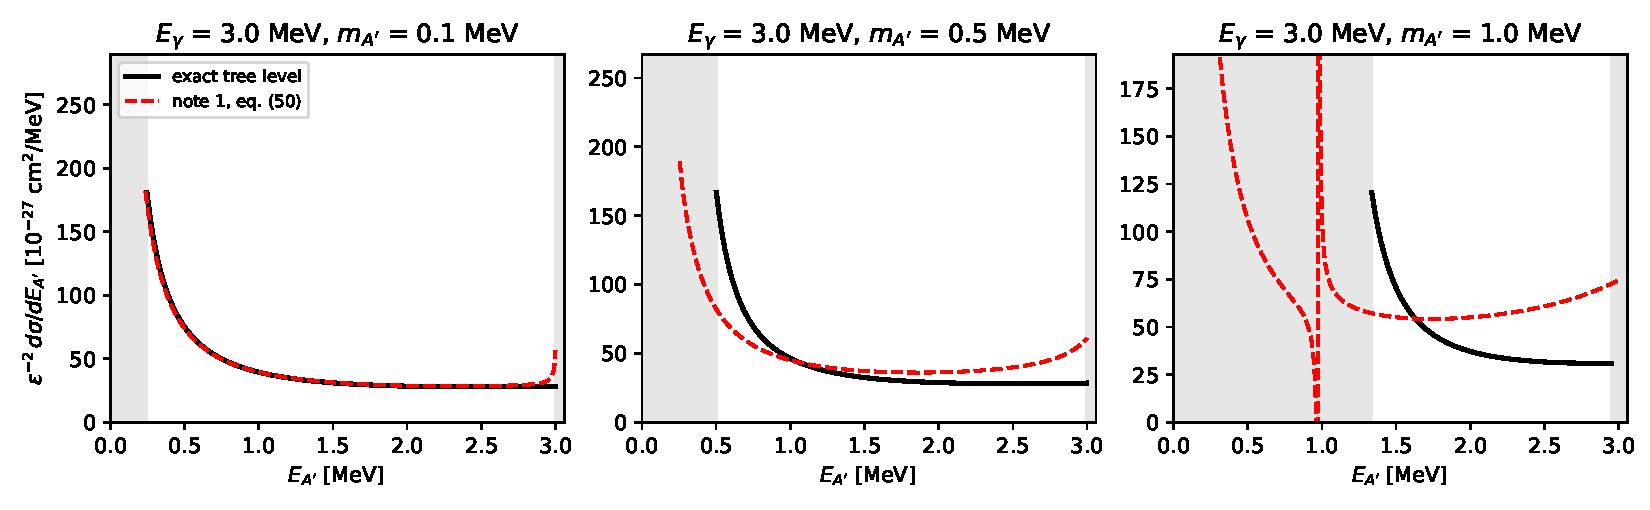
\includegraphics[width=\textwidth]{../work/fig_dsigma_dx_E3.pdf}
\caption{$\eps^{-2}\dd\sigma/\dd E_{\Ap}$ en $\omega=3$~MeV. Negro: exacta. Rojo a trazos: ec.~(50) del apunte sobre
el rango que el propio apunte declara. Gris: fuera del rango exacto $[x_-,x_+]$. En el panel derecho
($M=1$~MeV) se ve el polo de la ec.~\eqref{eq:polo} dentro de la zona gris.}
\end{figure}

\subsection{La prueba cruzada}
Para separar la responsabilidad de la fórmula de la del rango, basta cruzarlos:

\begin{center}\small
\begin{tabular}{@{}ll@{}}
\toprule
Qué se evalúa & Resultado\\
\midrule
Fórmula exacta, sobre el rango del apunte & aparece la misma discontinuidad\\
Fórmula del apunte, sobre el rango exacto $[x_-,x_+]$ & curva suave, sin polo (se aparta 0.48--2.36, sin rasgos)\\
\bottomrule
\end{tabular}
\end{center}

\noindent La discontinuidad es responsabilidad del \textbf{rango}, no de la fórmula.

\subsection{Por qué el rango exacto nunca lo toca}
\begin{equation}
\frac{\min_\omega x_-(\omega)}{M^2/2m_e}=10.4,\;2.04,\;1.26
\qquad\text{para } M=0.1,\;0.5,\;1~\text{MeV},
\end{equation}
siempre mayor que 1 (verificado hasta $M=1$~MeV). Hay una razón física: $b=0$ pone al electrón intercambiado
\emph{on-shell}, es decir el subproceso $e\to e+\Ap$ con las dos partículas reales. Eso está prohibido para partículas
libres, porque no se pueden conservar energía e impulso simultáneamente. La cinemática exacta lo sabe y nunca llega
ahí; la aproximada perdió esa información al borrar la masa del $\Ap$ de $|\vec k'|$.

Por eso la curva nueva de $M=1$~MeV en \texttt{cFig1\_new.png} arranca en $1.25$~MeV y baja monótona: no hay nada que
reparar en el polo, simplemente esa región ya no se visita.


%=====================================================================================================
\section{¿De dónde salen exactamente \texorpdfstring{$x_-$}{x-} y \texorpdfstring{$x_+$}{x+}? (deducción de la ec.~(5) del informe)}
%=====================================================================================================

\noindent\textbf{Respuesta corta.} De dos lugares, y dan lo mismo. (A) Son la energía del $\Ap$ en el CM,
$E^*=(s+M^2-m_e^2)/2\sqrt s$, boosteada al laboratorio con $\cos\theta^*=\pm1$. (B) Son las dos raíces de poner
$\cos\theta=\pm1$ en la relación \emph{exacta} ángulo--energía --- que es el mismo razonamiento del apunte, pero sin
haber borrado antes la masa del $\Ap$ de $|\vec k'|$. La ruta (B) es la que pedís: da una cuadrática en $\wpr$ cuyo
discriminante es $E^2\lambda(s,m_e^2,M^2)$, y de ahí sale la raíz de la ec.~(5). El precio de haber usado
$|\vec k'|\approx\wpr$ es que esa cuadrática degenera en una lineal y se pierde una de las dos raíces, junto con el
umbral.

\subsection{Ruta A: impulso de dos cuerpos en el CM, llevado al laboratorio}
En el centro de masa el estado final es de dos cuerpos, así que la energía y el impulso del $\Ap$ están fijados por
$s$ solo:
\begin{equation}
E^*_{\Ap}=\frac{s+M^2-m_e^2}{2\sqrt s},\qquad
|\vec q^{\,*}|=\frac{\sqrt{\lambda(s,m_e^2,M^2)}}{2\sqrt s},\qquad
\lambda(x,y,z)=x^2+y^2+z^2-2xy-2yz-2zx,
\end{equation}
y lo único libre es la dirección $\theta^*$. El CM se mueve respecto del laboratorio (electrón en reposo) con
\begin{equation}
\beta_{\rm cm}=\frac{E}{E+m_e},\qquad
\gamma_{\rm cm}=\frac{E+m_e}{\sqrt s},\qquad
\beta_{\rm cm}\gamma_{\rm cm}=\frac{E}{\sqrt s},\qquad s=m_e^2+2m_eE .
\end{equation}
La energía en el laboratorio es entonces una función \emph{lineal} de $\cos\theta^*$,
\begin{equation}
\wpr=\gamma_{\rm cm}E^*_{\Ap}+\beta_{\rm cm}\gamma_{\rm cm}\,|\vec q^{\,*}|\cos\theta^* ,
\end{equation}
de modo que sus extremos están en $\cos\theta^*=\pm1$ y no en ningún punto interior:
\begin{equation}
\boxed{\;x_\pm=\gamma_{\rm cm}E^*_{\Ap}\pm\beta_{\rm cm}\gamma_{\rm cm}|\vec q^{\,*}|
=\frac{(E+m_e)(s+M^2-m_e^2)\pm E\sqrt{\lambda(s,m_e^2,M^2)}}{2s}\;}
\label{eq:xpm}
\end{equation}
que es la ec.~(5) del informe. Nada acá depende de la dinámica: es cinemática de dos cuerpos, vale para cualquier
$\gamma e\to Xe$ con $m_X=M$.

\subsection{Ruta B: \texorpdfstring{$\cos\theta=\pm1$}{cos = +-1}, que es el argumento del apunte}
El apunte obtiene su rango pidiendo que el coseno del ángulo de salida llegue a sus valores extremos. Hagamos eso
mismo, pero con la relación exacta. De $(p+k-q)^2=m_e^2$, con $|\vec k'|=\sqrt{\wpr^{\,2}-M^2}$,
\begin{equation}
M^2+2m_e(E-\wpr)-2E\big(\wpr-|\vec k'|\cos\theta\big)=0
\quad\Longrightarrow\quad
\cos\theta=\frac{(\wpr-m_e)E+m_e\wpr-M^2/2}{E\,|\vec k'|}.
\label{eq:cos}
\end{equation}
Poner $\cos\theta=\pm1$ deja
\begin{equation}
\underbrace{M^2+2m_eE-2(m_e+E)\,\wpr}_{\textstyle \equiv\,A(\wpr)}=\mp\,2E\sqrt{\wpr^{\,2}-M^2}\, .
\label{eq:Aform}
\end{equation}
Elevando al cuadrado, los dos signos colapsan en una \emph{única} cuadrática $A^2-4E^2(\wpr^2-M^2)=0$:
\begin{equation}
4s\,\wpr^{\,2}-4(E+m_e)\big(s+M^2-m_e^2\big)\wpr+\big(M^2+2m_eE\big)^2+4E^2M^2=0 ,
\label{eq:quad}
\end{equation}
donde el coeficiente cuadrático salió $4[(E+m_e)^2-E^2]=4(m_e^2+2m_eE)=4s$ y se usó $M^2+2m_eE=s+M^2-m_e^2$. Su
discriminante es
\begin{equation}
16(E+m_e)^2(s+M^2-m_e^2)^2-16s\Big[(s+M^2-m_e^2)^2+4E^2M^2\Big]
=16E^2\Big[(s+M^2-m_e^2)^2-4sM^2\Big]=16E^2\lambda(s,m_e^2,M^2),
\end{equation}
usando otra vez $(E+m_e)^2-s=E^2$ y la identidad $\lambda(s,m_e^2,M^2)=(s+M^2-m_e^2)^2-4sM^2$. Las dos raíces de
\eqref{eq:quad} son por lo tanto \emph{exactamente} $x_\pm$ de la ec.~\eqref{eq:xpm}. Es decir: el argumento del
apunte es correcto; lo que estaba mal era la relación \eqref{eq:cos} sobre la que se lo aplicaba.

\medskip
\noindent\textbf{Dónde se pierde la segunda raíz con $|\vec k'|\approx\wpr$.} Con $M\to0$ dentro de
$|\vec k'|$ pero no en el resto, el término $4E^2M^2$ del lado derecho de \eqref{eq:Aform} desaparece y
\eqref{eq:quad} se vuelve $A(\wpr)^2=4E^2\wpr^{\,2}$, o sea $A=\pm2E\wpr$: dos ecuaciones \emph{lineales}, cada una
con una sola solución, y ninguna condición sobre el discriminante. Por eso en el apunte el rango no tiene umbral: la
raíz cuadrada que lo lleva adentro ya no está.

\subsection{Cuál raíz es cuál (y por qué ninguna es espuria)}
Elevar al cuadrado puede inventar soluciones, así que hay que mirar el signo de $A$ en \eqref{eq:Aform}: la raíz con
$A<0$ corresponde a $\cos\theta=+1$ y la de $A>0$ a $\cos\theta=-1$. Evaluando, $A(x_+)<0$ \emph{siempre}: el
extremo superior es emisión hacia adelante, como en Compton. El extremo inferior, en cambio, es hacia atrás sólo si
el $\Ap$ le gana al CM, $\beta^*_{\Ap}>\beta_{\rm cm}$, que se reduce (sympy) a una condición lineal en $E$:
\begin{equation}
\frac{\sqrt\lambda}{s+M^2-m_e^2}>\frac{E}{E+m_e}
\iff \big(M^2+2m_eE\big)^2>4M^2(E+m_e)^2
\iff 2E(m_e-M)>M(2m_e-M).
\label{eq:cono}
\end{equation}
Para $M\ge m_e$ es imposible, y para $M<m_e$ pide $E>E_b\equiv M(2m_e-M)/2(m_e-M)$: $E_b=0.1122$~MeV para
$M=0.1$~MeV (apenas por encima del umbral $0.1098$) pero $E_b=11.87$~MeV para $M=0.5$~MeV. Por debajo de $E_b$
\emph{las dos} raíces tienen $\cos\theta=+1$ y la emisión está confinada a un cono hacia adelante: en $E=3$~MeV,
$\theta\le67.4^\circ$ para $M=0.5$~MeV y $\theta\le17.4^\circ$ para $M=1$~MeV. Ninguna raíz es espuria --- las dos
salen de la misma rama de \eqref{eq:Aform} --- y $x_\pm$ siguen siendo los extremos, porque el boost de la ruta A no
se entera de nada de esto. \textbf{La lectura "$x_-$ es el $\Ap$ emitido hacia atrás" vale sólo en el régimen
\eqref{eq:cono};} en el reactor, con $M\gtrsim0.5$~MeV y $E\lesssim8$~MeV, no vale.

\subsection{Los dos controles de la fórmula}
\textbf{(i) $M\to0$ devuelve el rango del apunte.} $\lambda\to(s-m_e^2)^2=(2m_eE)^2$ y
\begin{equation}
x_+\to E,\qquad x_-\to\frac{E}{1+2E/m_e},
\end{equation}
que son las ecs.~(24)--(25) del apunte, es decir el retroceso Compton. El rango del apunte no es una aproximación al
exacto: es su límite de masa cero, sin ninguna dependencia en $M$.

\smallskip
\noindent\textbf{(ii) El umbral sale solo.} $x_\pm$ son reales sólo si $\lambda\ge0$, o sea $s\ge(m_e+M)^2$:
\begin{equation}
E\ge E_{\rm th}=M+\frac{M^2}{2m_e},
\end{equation}
y en el umbral las dos raíces se juntan en $x_+=x_-=M(E_{\rm th}+m_e)/(m_e+M)$ --- el $\Ap$ en reposo en el CM. En el
apunte el umbral no aparece porque su rango, al ser el límite $M\to0$, existe para todo $E$.

\subsection{Números}
\begin{center}\small
\begin{tabular}{@{}lccc@{}}
\toprule
$M$ [MeV] & 0.1 & 0.5 & 1.0\\
\midrule
$E_{\rm th}=M+M^2/2m_e$ [MeV] & 0.1098 & 0.7446 & 1.9785\\
$x_\pm$ en el umbral [MeV] & 0.1016 & 0.6210 & 1.6476\\
$[x_-,x_+]$ en $E=3$ MeV [MeV] & $[0.2460,\;3.0000]$ & $[0.5011,\;2.9981]$ & $[1.3359,\;2.9548]$\\
$\min_E x_-/(M^2/2m_e)$ & 10.54 & 2.04 & 1.26\\
\bottomrule
\end{tabular}
\end{center}
\noindent El rango del apunte, $[0.2354,\;3.0000]$~MeV en $E=3$~MeV, es el mismo para las tres masas. La última fila
es la que importa para la Sección~1: el polo del canal $u$ en $\wpr=M^2/2m_e$ queda siempre afuera, por un factor que
nunca baja de $1.14$ (mínimo sobre $M\le1.4$~MeV y $E\le60$~MeV).

\subsection{Verificación}
\texttt{work/check\_xpm.py} (corrido; salida en \texttt{work/check\_xpm.log} y
\texttt{work/check\_xpm\_out.json}), termina en \texttt{ALL ASSERTIONS PASSED}:
\begin{itemize}\itemsep2pt
\item ruta A $=$ ec.~\eqref{eq:xpm} y ruta B $=$ ec.~\eqref{eq:xpm}, ambas como identidades simbólicas
(\texttt{sympy}, \texttt{simplify(...) == 0}); también los coeficientes de \eqref{eq:quad} y que el discriminante es
$16E^2\lambda$;
\item $\cos\theta(x_\pm)=\pm1$ a $2.4\times10^{-9}$ en 296 puntos $(E,M)$, con el signo que predice
\eqref{eq:cono} en cada uno (169 con $x_-$ hacia atrás, 127 en régimen de cono);
\item $|\cos\theta|>1$ en 1184 puntos de prueba fuera de $[x_-,x_+]$: el intervalo no es una elección, es todo lo que
hay;
\item los límites $M\to0$ con \texttt{sympy.limit}, y $\lambda=0\Leftrightarrow E=E_{\rm th}$ con \texttt{sympy.solve}.
\end{itemize}
\noindent \textbf{Lo que no está chequeado acá:} que $\lambda\ge0$ sea el único requisito físico (no se comprobó
positividad del espacio de fases de tres cuerpos, porque no hay tres cuerpos), y el régimen $M>2m_e$, donde el $\Ap$
puede decaer a $e^+e^-$ y esta cinemática de producción sigue valiendo pero la detección no. El barrido numérico llega
a $M=1.4$~MeV y $E=60$~MeV.


%=====================================================================================================
\section{¿Por qué la Figura 1 pica en \texorpdfstring{$\wpr\to m_{\Ap}$}{w' -> mA'} al incorporar \texttt{wp\_production\_new\_f}?}
%=====================================================================================================

\noindent\textbf{Respuesta corta.} Porque la grilla nueva es una de tres piezas y las otras dos siguen siendo las
viejas. La ec.~(50) del apunte \emph{tiene un polo simple en} $\wpr=m_{\Ap}$ --- destapado por la misma corrección de
\texttt{cos\_theta\_f} --- y \texttt{Rw\_f} no declara vacía esa región. La grilla vieja arrancaba en $m_{\Ap}/2$,
\emph{por debajo} de la masa, donde el coseno exacto da \texttt{NaN} y el guard de \texttt{Rw\_f} devolvía ceros: el
polo nunca se muestreaba. \texttt{wp\_production\_new\_f} pone su primer punto en $m_{\Ap}(1+10^{-4})$, justo encima.
No es un problema de la grilla: es que \texttt{wp\_production\_new\_f}, \texttt{Rw\_new\_f} y \texttt{ds\_dwp\_new\_f}
son un conjunto.

\subsection{La ec.~(50) diverge en $\wpr=m_{\Ap}$}
El corchete de \texttt{ds\_dwp\_f} lleva el ángulo de salida escrito explícitamente,
\begin{equation}
\texttt{ket}=\frac{\wpr}{\omega}+\frac{\omega}{\wpr}+m_{\Ap}^2 f_{su}+\cos^2\theta-1 ,
\end{equation}
y el $\cos\theta$ corregido tiene $|\vec k'|=\sqrt{\wpr^{\,2}-m_{\Ap}^2}$ en el denominador (ec.~\eqref{eq:cos}).
Entonces
\begin{equation}
\cos\theta\;\xrightarrow[\wpr\to m_{\Ap}]{}\;\frac{(m_{\Ap}-m_e)\omega+m_e m_{\Ap}-m_{\Ap}^2/2}{\omega\sqrt{\wpr^{\,2}-m_{\Ap}^2}}
\sim(\wpr-m_{\Ap})^{-1/2}
\quad\Longrightarrow\quad
\frac{\dd\sigma}{\dd\wpr}\Big|_{(50)}\sim\frac{1}{\wpr-m_{\Ap}} .
\end{equation}
Medido en $\omega=3$~MeV, el exponente log--log ajustado es $-1.000$ para las tres masas. La sección eficaz exacta no
tiene ningún ángulo adentro --- $F$ depende sólo de $a,b,c,d$ --- y ahí tiende a una constante (exponente $<10^{-6}$
en valor absoluto). \textbf{El polo es de la fórmula del apunte, no de la cinemática nueva:} lo único que hizo la
corrección de \texttt{cos\_theta\_f} fue devolverle al coseno la masa que la ec.~(20) le había borrado, y con ella la
divergencia que el apunte no veía.

\subsection{\texttt{Rw\_f} no protege esa región}
\texttt{invwpmin\_f} devuelve $+\infty$ para $\wpr\ge m_e/2=0.2555$~MeV, así que \texttt{Rw\_f} entrega el rango
completo $[\wpr,\omega_{\max}]$ y nunca es vacío. El dominio exacto, $\{\omega:\;x_-(\omega)\le\wpr\le x_+(\omega)\}$,
dice otra cosa (en $\wpr=1.0001\,m_{\Ap}$, con $\omega_{\max}=10$~MeV):

\begin{center}\small
\begin{tabular}{@{}lll@{}}
\toprule
$m_{\Ap}$ [MeV] & \texttt{Rw\_f} (viejo) & \texttt{Rw\_new\_f} (exacto)\\
\midrule
0.1 & $\omega\in[0.100,\,0.148]$ & $[0.112,\,0.113]$ --- el 1.5\,\% del ancho\\
0.5 & $[0.500,\,10.0]$ & $[7.24,\,10.0]$ --- sólo los $\gamma$ más energéticos (29\,\%)\\
1.0 & $[1.000,\,10.0]$ & \textbf{vacío}: no hay nada por debajo de $\min_\omega x_-=1.2547$~MeV\\
\bottomrule
\end{tabular}
\end{center}

\noindent Esos puntos reciben entonces todo el flujo de gammas de baja energía --- donde el espectro del reactor es
máximo --- multiplicado por un integrando que está divergiendo. Dentro del dominio exacto eso es imposible:
$|\cos\theta|\le1$ por construcción, porque $x_\pm$ \emph{son} los puntos donde $\cos\theta=\pm1$ (Sección~2). Se
verificó: $|\cos\theta|\le0.9641$ en el dominio exacto de $m_{\Ap}=0.1$~MeV en ese mismo $\wpr$.

\subsection{Por qué antes no se veía}
\texttt{wp\_production\_OLD\_f} arrancaba en $m_{\Ap}/2$: $0.0510$, $0.2510$ y $0.5010$~MeV para
$m_{\Ap}=0.1,\,0.5,\,1$~MeV, las tres \emph{por debajo de la masa}. Con el coseno exacto eso es la raíz de un número
negativo (\texttt{NaN}), o lo mata el guard \texttt{min\_val <= wp} de \texttt{Rw\_f}; y el primer punto por encima de
$m_{\Ap}$ caía lejos del polo (con \texttt{wpsize}~$=10$, a $\sim1$~MeV). La grilla nueva pone el primero a
$10^{-4}$ del borde: $\wpr=0.10099$, $0.50095$ y $1.00090$~MeV.

\subsection{Números, y el diagnóstico de un minuto}
Crecimiento de la ec.~(50) entre $\wpr=1.01\,m_{\Ap}$ y $1.0001\,m_{\Ap}$, en $\omega=3$~MeV: $\times975$
($m_{\Ap}=0.1$), $\times39$ ($0.5$), $\times699$ ($1.0$). En el primer punto de la grilla, $\omega=3$~MeV,
$\eps=1$: ec.~(50) $=1.11\times10^{-21}$~cm$^2$/MeV contra $7.49\times10^{-25}$ de la exacta ($m_{\Ap}=0.1$~MeV).

\medskip
\noindent\textbf{Cómo confirmarlo en un minuto:} cambiar \texttt{delta\_frac} de $10^{-4}$ a $10^{-5}$ y volver a
graficar. La altura del pico se multiplica por $\sim10$ y el resto de la curva no se mueve (verificado: $\times10.0$
por década en las tres masas, ya en el régimen asintótico del polo). \emph{La física no depende del espaciado de la
grilla; un polo $1/(\wpr-m_{\Ap})$ muestreado más cerca, sí.}

\subsection{El arreglo}
Las tres piezas van juntas. De menor a mayor:
\begin{enumerate}\itemsep2pt
\item \textbf{Mínimo:} reemplazar también \texttt{Rw\_f} por \texttt{Rw\_new\_f}. Sola alcanza para matar el pico,
porque restringe $(\omega,\wpr)$ al conjunto donde $|\cos\theta|\le1$. Pero deja la ec.~(50), que sigue estando mal
en el interior del rango (hasta un factor 2, informe Sección~7).
\item \textbf{Correcto:} \texttt{Rw\_new\_f} \emph{y} \texttt{ds\_dwp\_new\_f}. La curva de $m_{\Ap}=1$~MeV arranca
en $1.25$~MeV y baja monótona.
\item \textbf{Si se quiere conservar la ec.~(50) para comparar:} usarla con la grilla vieja
(\texttt{wp\_production\_OLD\_f}), no con la nueva.
\end{enumerate}

\subsection{Verificación}
\texttt{work/check\_wp\_production\_spike.py} (corrido; \texttt{work/check\_wp\_production\_spike.log}), que
reimplementa en python las tres funciones tal como están hoy en \texttt{mycodes/DP3\_Danilov.C}; termina en
\texttt{ALL ASSERTIONS PASSED}. Se asserta el exponente $-1$ de la ec.~(50) y el $0$ de la exacta, que
$|\cos\theta|\le1$ en el dominio exacto, que el dominio exacto es vacío en $m_{\Ap}=1$~MeV donde el viejo no lo es,
que los tres arranques de la grilla vieja están por debajo de $m_{\Ap}$, y el escaleo $\times10$ por década con
\texttt{delta\_frac}.

\smallskip
\noindent\textbf{Lo que no está chequeado:} no se corrió \texttt{DP3\_Danilov.C} en ROOT, así que la altura del pico
\emph{en esa figura} no está reproducida --- lo que está demostrado es el mecanismo y su escaleo con
\texttt{delta\_frac}. Tampoco se revisó si las otras curvas del macro (absorción, exclusión) usan el mismo par
grilla/dominio.

% =====================================================================================================
% Próximas preguntas: agregar una \section por cada una, con el mismo formato
% (respuesta corta -> desarrollo -> números -> verificación).
% Candidatas pendientes: por qué descartar los términos en me^2 rompe Klein-Nishina ; el jacobiano ;
% la normalización por electrón. (El umbral E_th quedó cubierto en la seccion 2; x_pm es la seccion 2.)
% =====================================================================================================

\end{document}
